\section{Impact of electronic noise on hit rates}
\label{sec:electronicnoise}

The hit rates presented in the main body of the note include all reported hits, including those from electronic noise. The contribution from electronic noise is detector-dependent, hence the inclusive hit rate is less useful for projecting to future LHC conditions because new detectors (sTGC, MM) will be deployed in the NSW. This appendix reports the hit rates with hit quality criteria cuts (\textit{ADC cuts}) which remove a large fraction of electronic noise while maintaining high efficiency for hits from incident particles. This is a more accurate reflection of the conditions for future MS detectors, though a proper unfolding to particle fluxes is still not attempted. The quality cuts considered for suppressing electronic noise are shown in Table~\ref{tab:electronic-adc}.

\begin{table}
  \begin{center}
    \begin{tabular}{c|c}
      detector & quality criteria \\
      \hline
      MDT      & tube ADC greater than 50 \\
      CSC      & both cluster secondary strips ($q_\text{left}$, $q_\text{right}$) greater than 0 \\
    \end{tabular}
    \caption{Criteria for a MDT tube hit or CSC cluster passing noise thresholds.}
    \label{tab:electronic-adc}
  \end{center}
\end{table}

\begin{table}
  \begin{center}
    \renewcommand{\arraystretch}{1.4}
    \begin{tabular}{c|c|c}
      figure                              & inclusive                                     & quality criteria \\
      \hline
      hit rates per region                & Fig.~\ref{fig:hitrates-vs-region-raw}              & Fig.~\ref{fig:hitrates-vs-region-adc} \\
      CSC hit rates vs. inst. lumi.       & Fig.~\ref{fig:hitrates-vs-lumi-csc-raw}            & Fig.~\ref{fig:hitrates-vs-lumi-csc-adc} \\
      hit rates vs. $r$                   & Fig.~\ref{fig:hitrates-vs-r-raw}                   & Fig.~\ref{fig:hitrates-vs-r-adc} \\
      fitted slopes vs. N(bunches)        & Fig.~\ref{fig:extrapolations-slope-vs-bunches-raw} & Fig.~\ref{fig:extrapolations-slope-vs-bunches-adc} \\
      projected hit rates vs. inst. lumi. & Fig.~\ref{fig:extrapolations-hitrates-adc}         & Fig.~\ref{fig:extrapolations-hitrates-adc} \\
    \end{tabular}
    \caption{Figures reported the inclusive hit rates and their equivalent figures reported with quality criteria requirements.}
    \label{tab:electronic-rawvsadc}
  \end{center}
\end{table}

\begin{figure}
  \begin{center}
    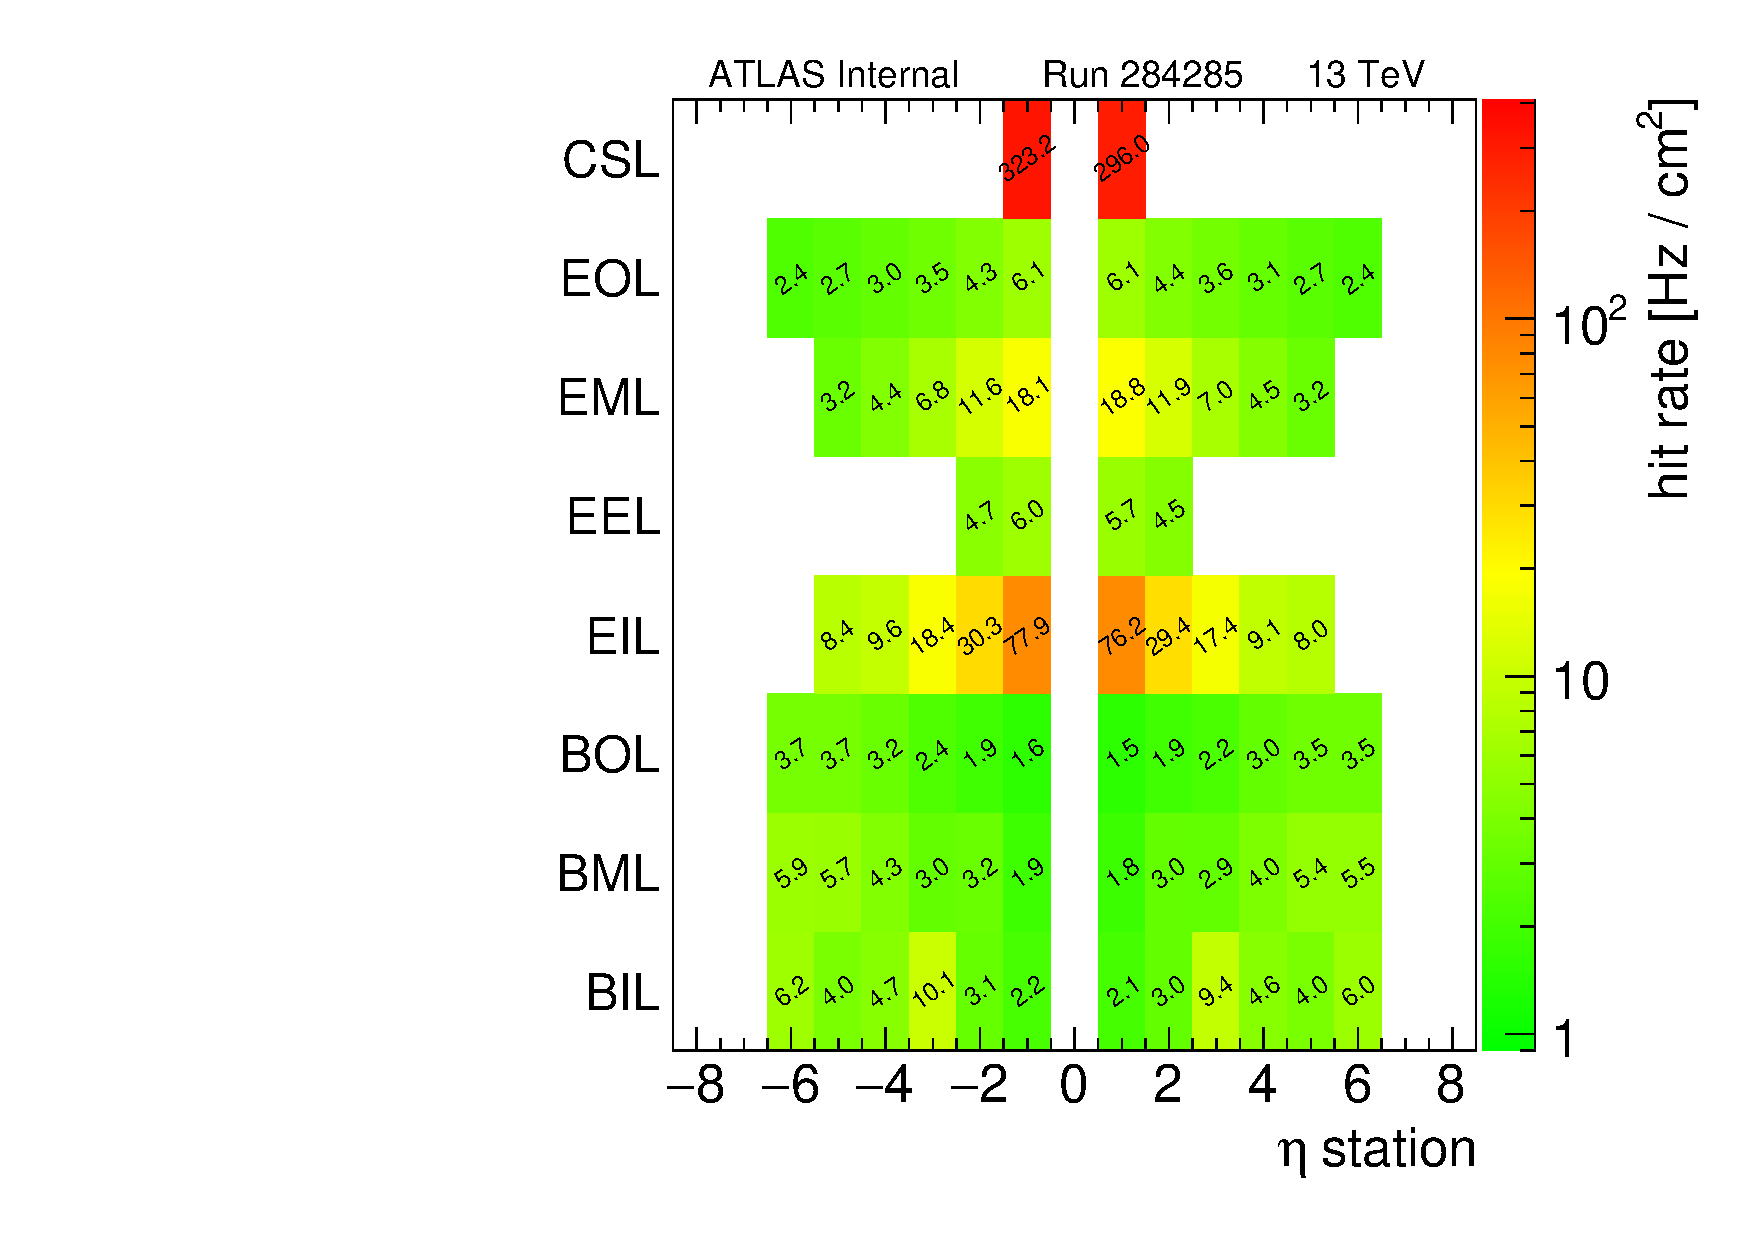
\includegraphics[width=0.45\textwidth]{./figures/rate_adc_vs_region_L_00284285.pdf}
    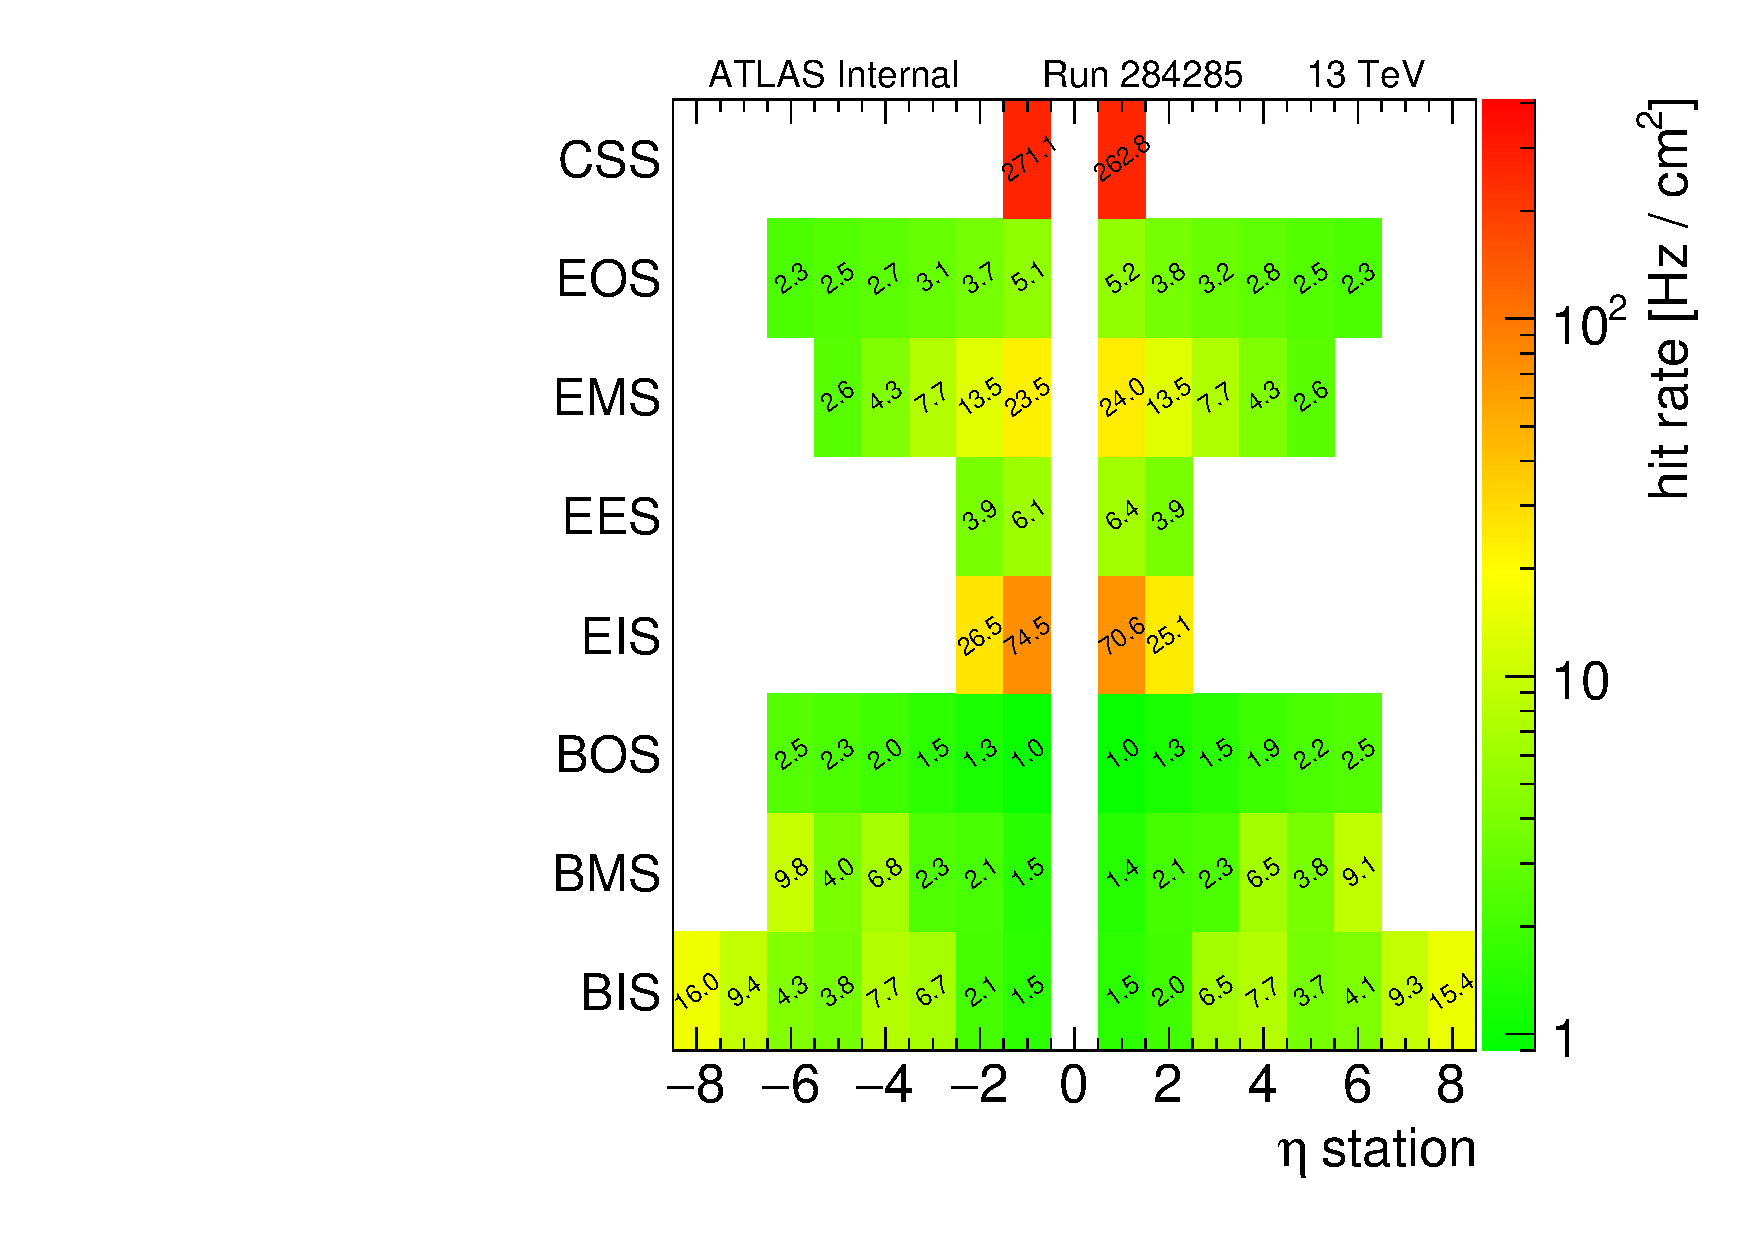
\includegraphics[width=0.45\textwidth]{./figures/rate_adc_vs_region_S_00284285.pdf}
    \caption{Total hit rate in the MDTs in Run 284285 in the largest regions of the detector. The rates are split into large sectors (left) and small sectors (right). Positive eta stations indicate the $+z$ side of ATLAS, and negative eta stations indicate the $-z$ side.}
    \label{fig:hitrates-vs-region-adc}
  \end{center}
\end{figure}

\begin{figure}
  \begin{center}
    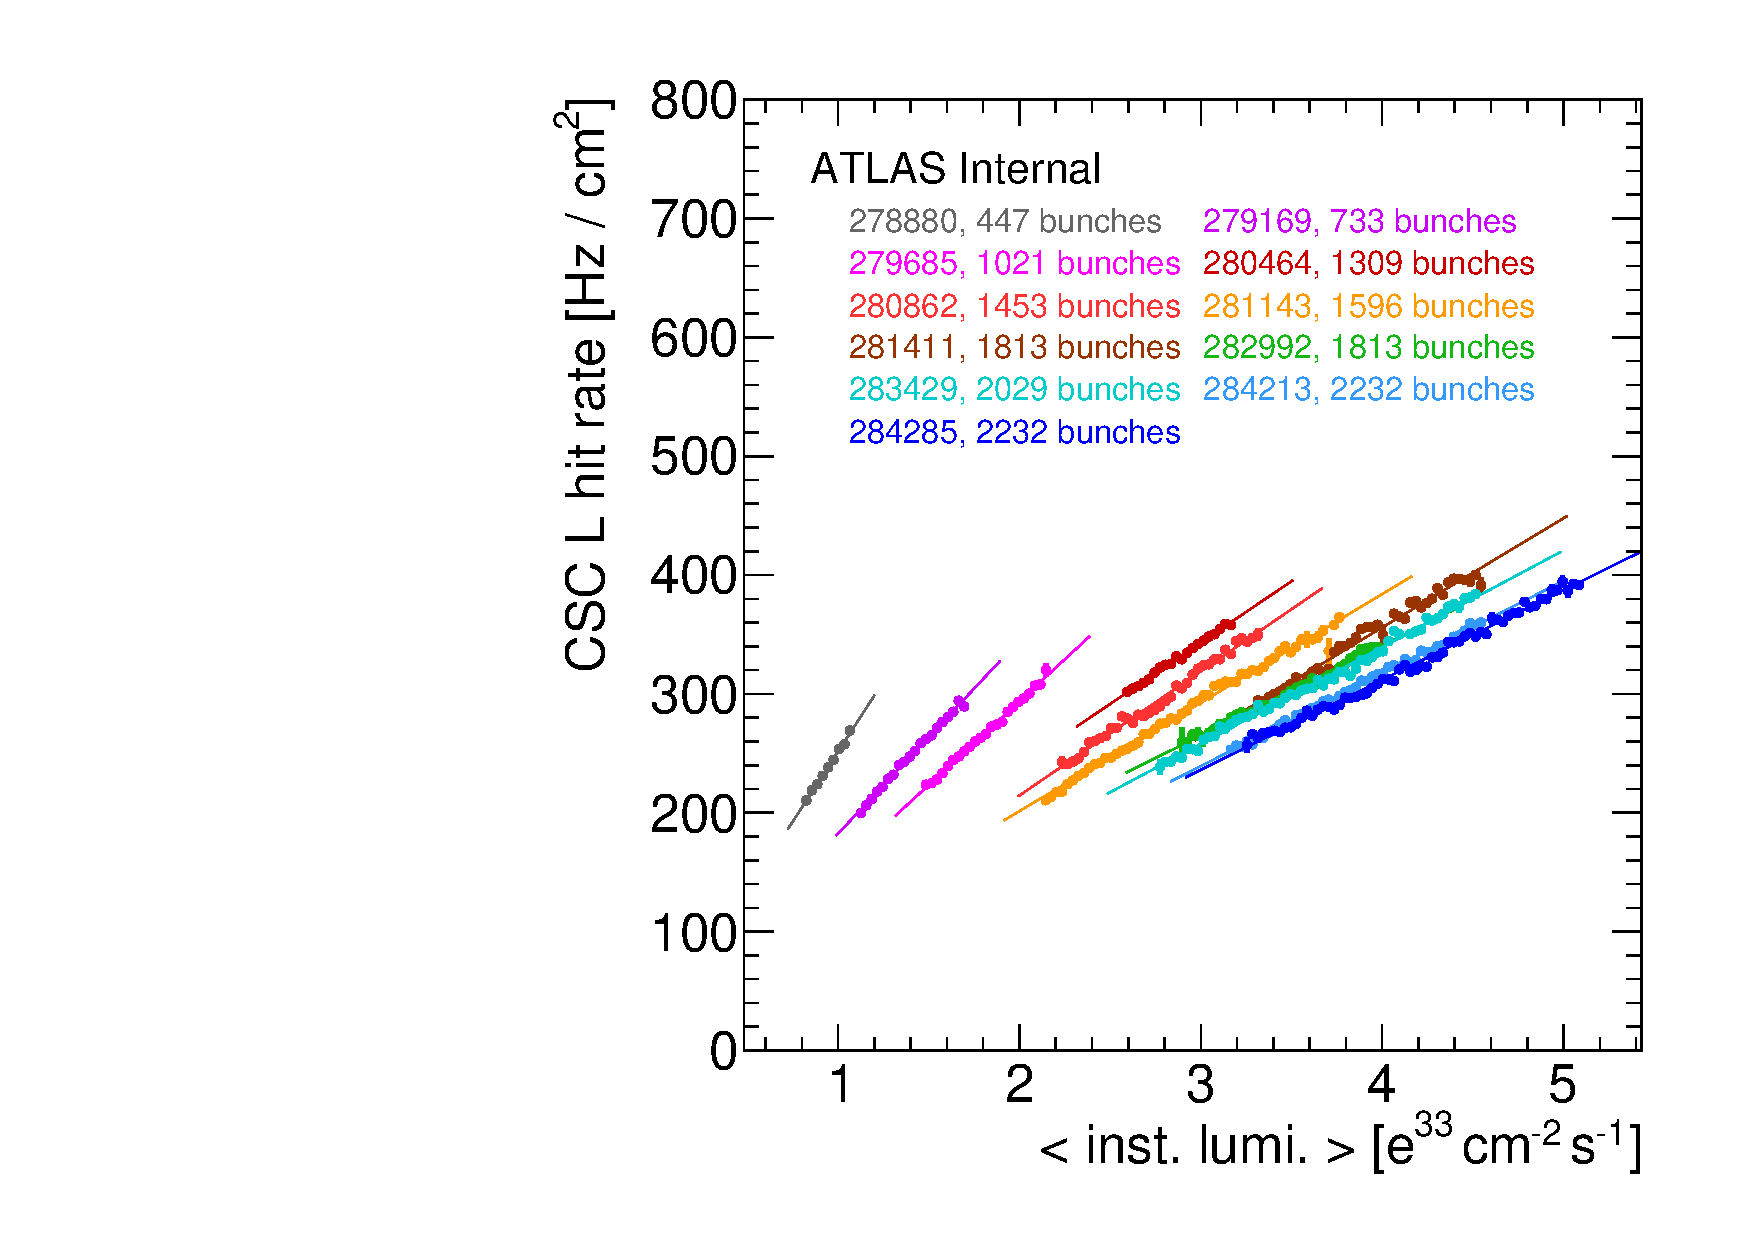
\includegraphics[width=0.45\textwidth]{./figures/rate_adc_vs_lumi_vs_evts_csc_CSL1_overlay.pdf}
    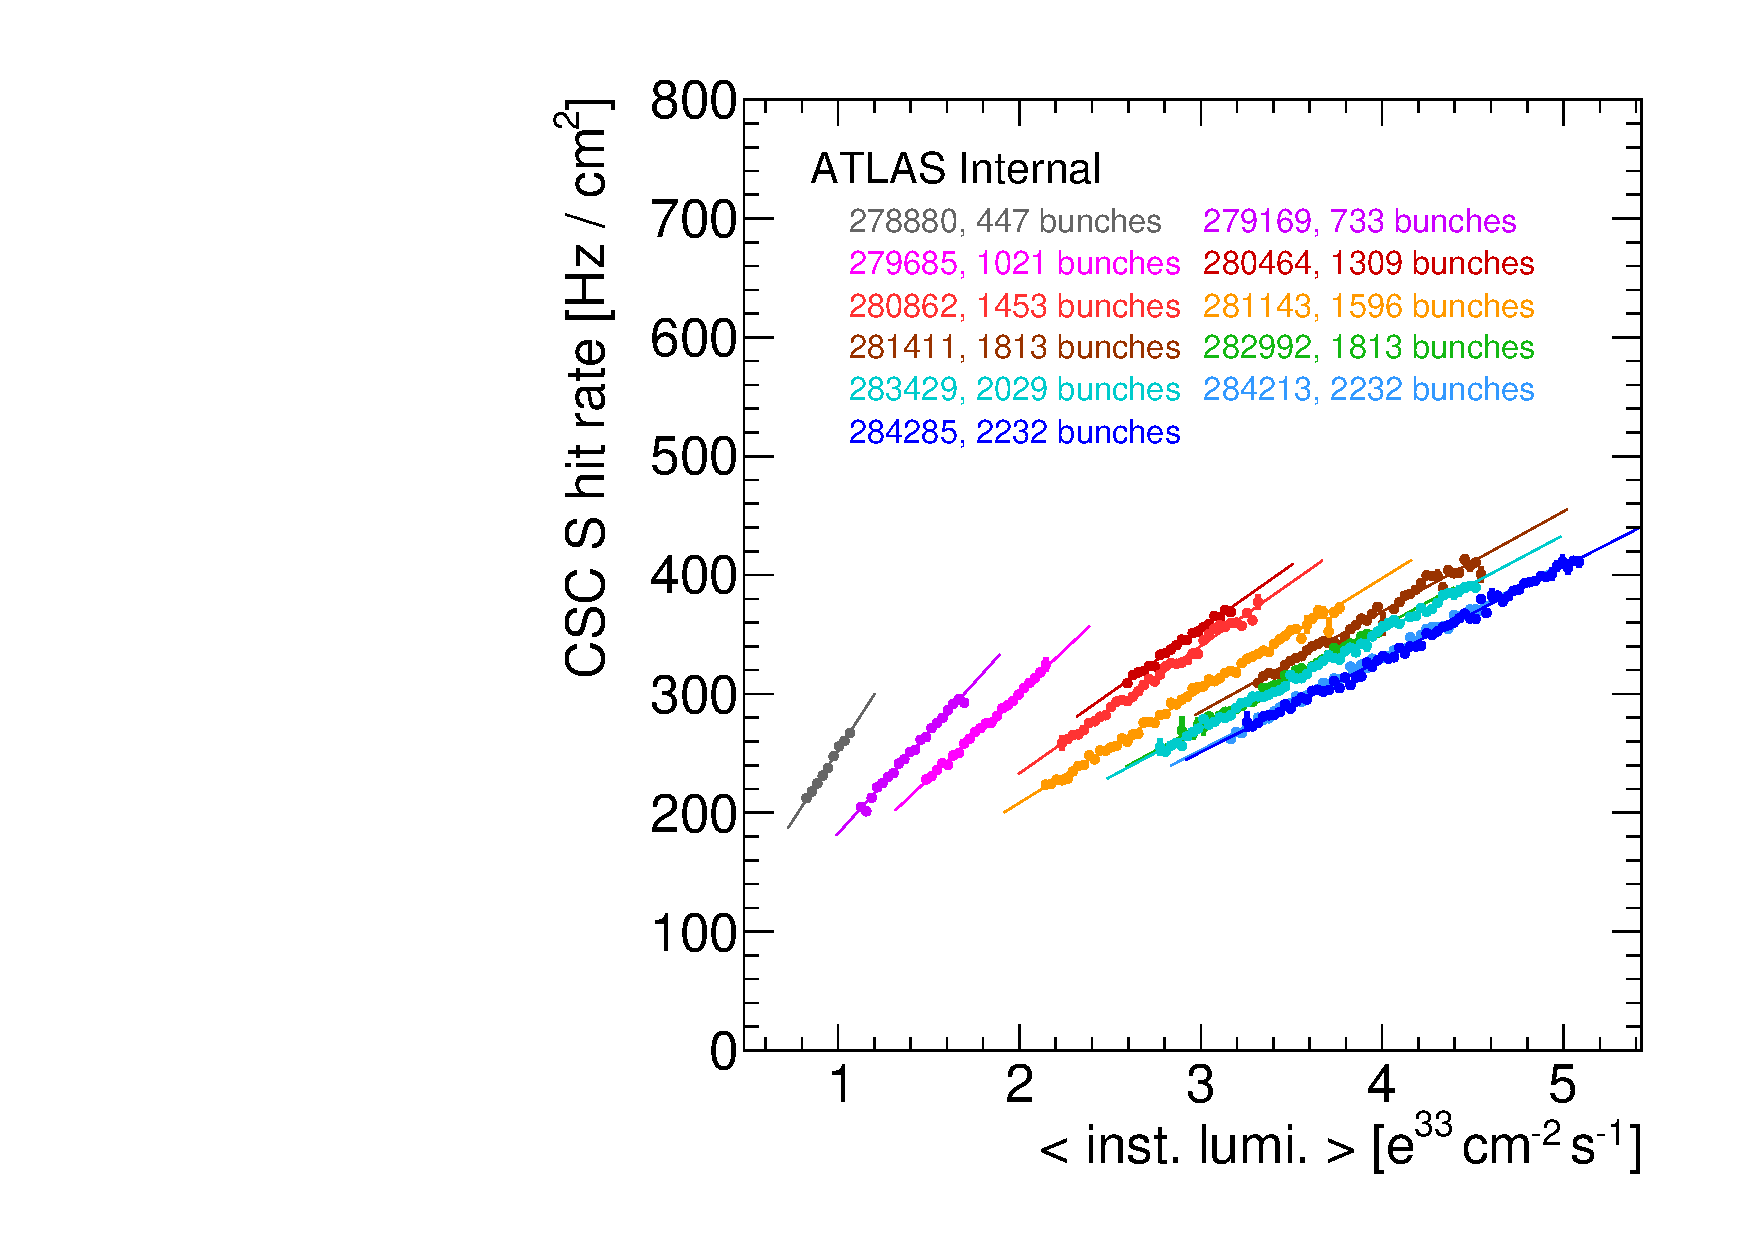
\includegraphics[width=0.45\textwidth]{./figures/rate_adc_vs_lumi_vs_evts_csc_CSS1_overlay.pdf}
    \caption{Total hit rate in the CSC large (left) and small (right) chambers as a function of instantaneous luminosity, for multiple runs.}
    \label{fig:hitrates-vs-lumi-csc-adc}
  \end{center}
\end{figure}

\begin{figure}
  \begin{center}
    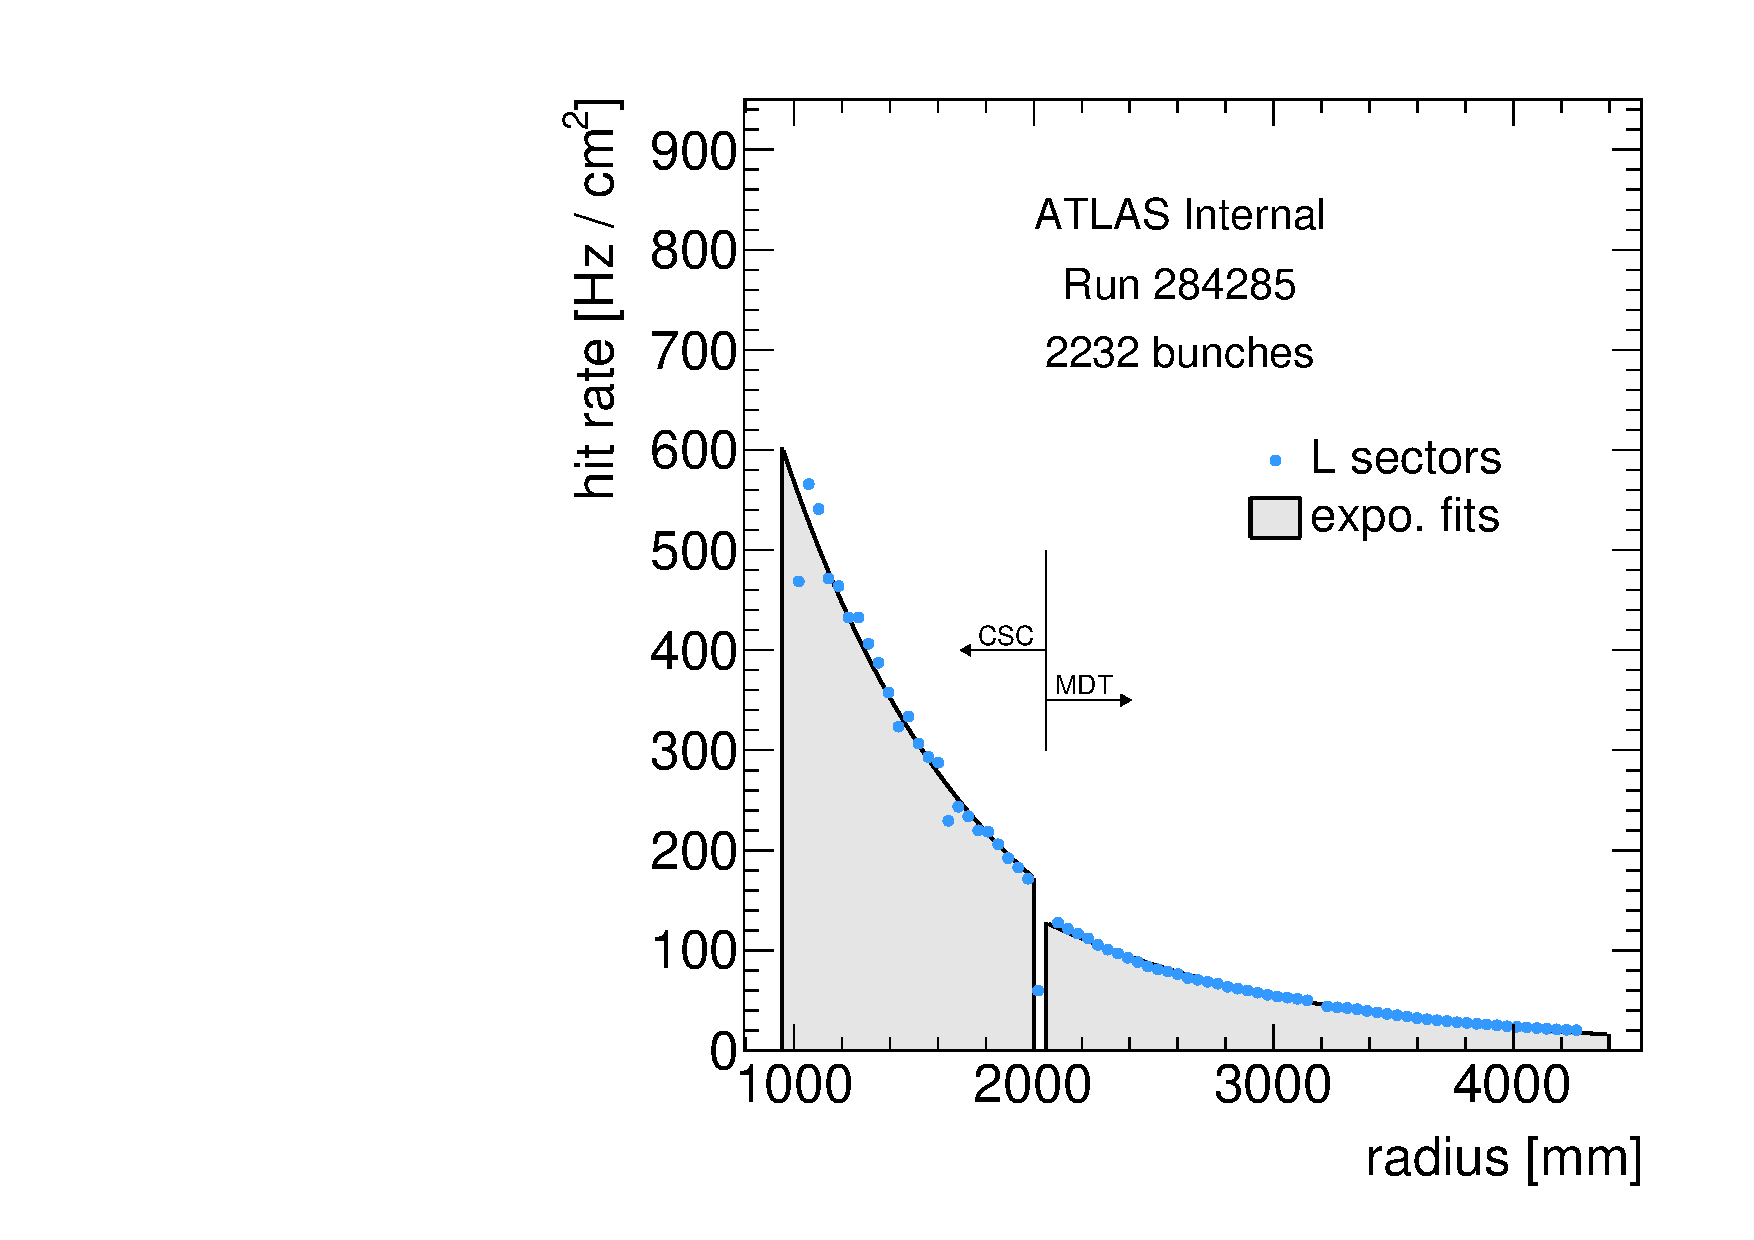
\includegraphics[width=0.45\textwidth]{./figures/rate_adc_vs_r_L_00284285.pdf}
    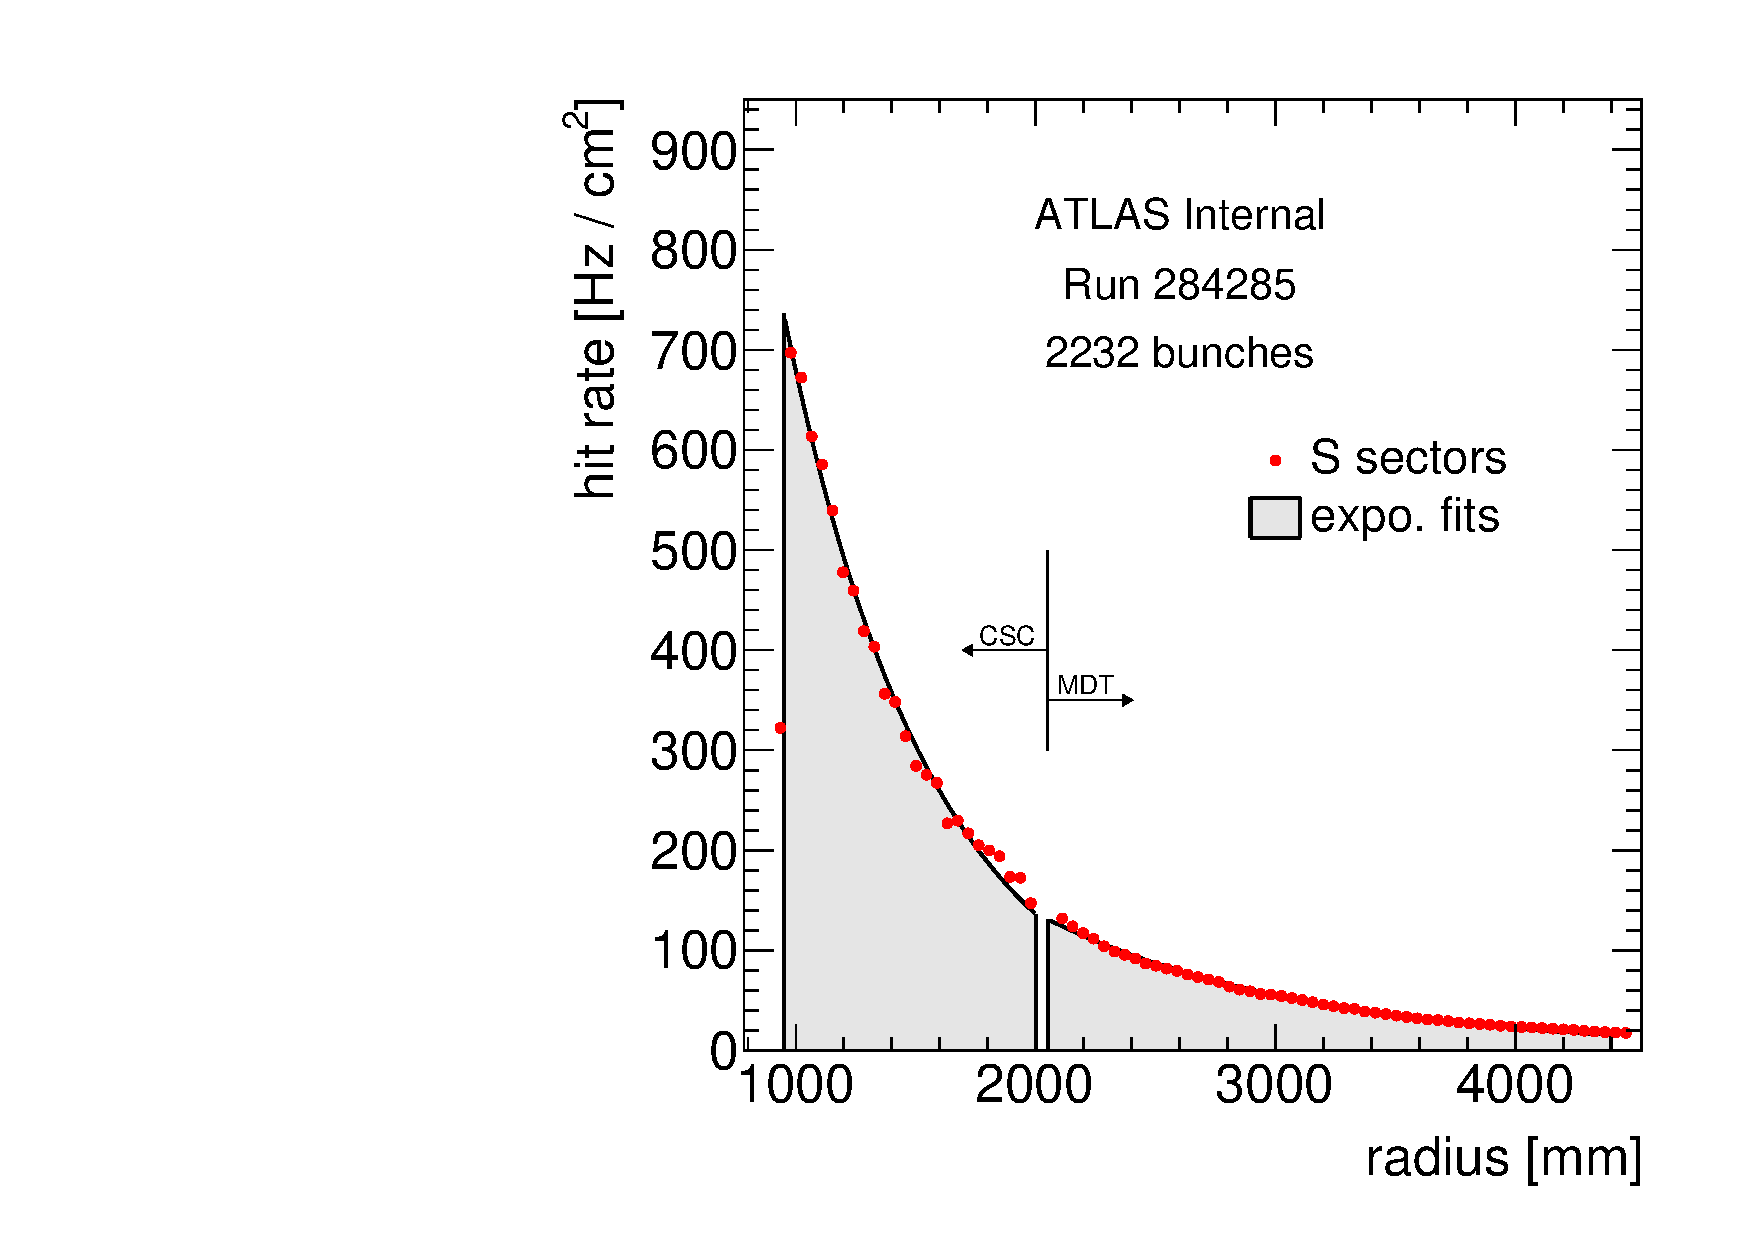
\includegraphics[width=0.45\textwidth]{./figures/rate_adc_vs_r_S_00284285.pdf}
    \caption{Total hit rate as a function of the transverse distance from the beam pipe in the small wheel, for large (left) and small (right) sectors, in Run 284285.}
    \label{fig:hitrates-vs-r-adc}
  \end{center}
\end{figure}

\begin{table}
  \begin{center}
    \renewcommand{\arraystretch}{1.4}
    \begin{tabular}{c|c|c|c}
      \multicolumn{1}{c|}{}              & \multicolumn{2}{c|}{\rate}                               & \multicolumn{1}{c}{} \\
      \hspace{0.6cm}region\hspace{0.6cm} & \hspace{0.6cm}average\hspace{0.6cm} & peak: smallest $r$ & peak / average \\
      \hline\hline
      CSC L                              & 310                                 & 601                & 1.94 \\
      CSC S                              & 324                                 & 738                & 2.28 \\
    \end{tabular}
    \caption{Comparison of the CSC chamber average hit rate with the hit rate closest to the beampipe in Run 284285. The average luminosity in Run 284285 is $\mathcal{L}=4.1\times10^{33}$.}
    \label{tab:hitrates-vs-r-adc}
  \end{center}
\end{table}

\begin{figure}
  \begin{center}
    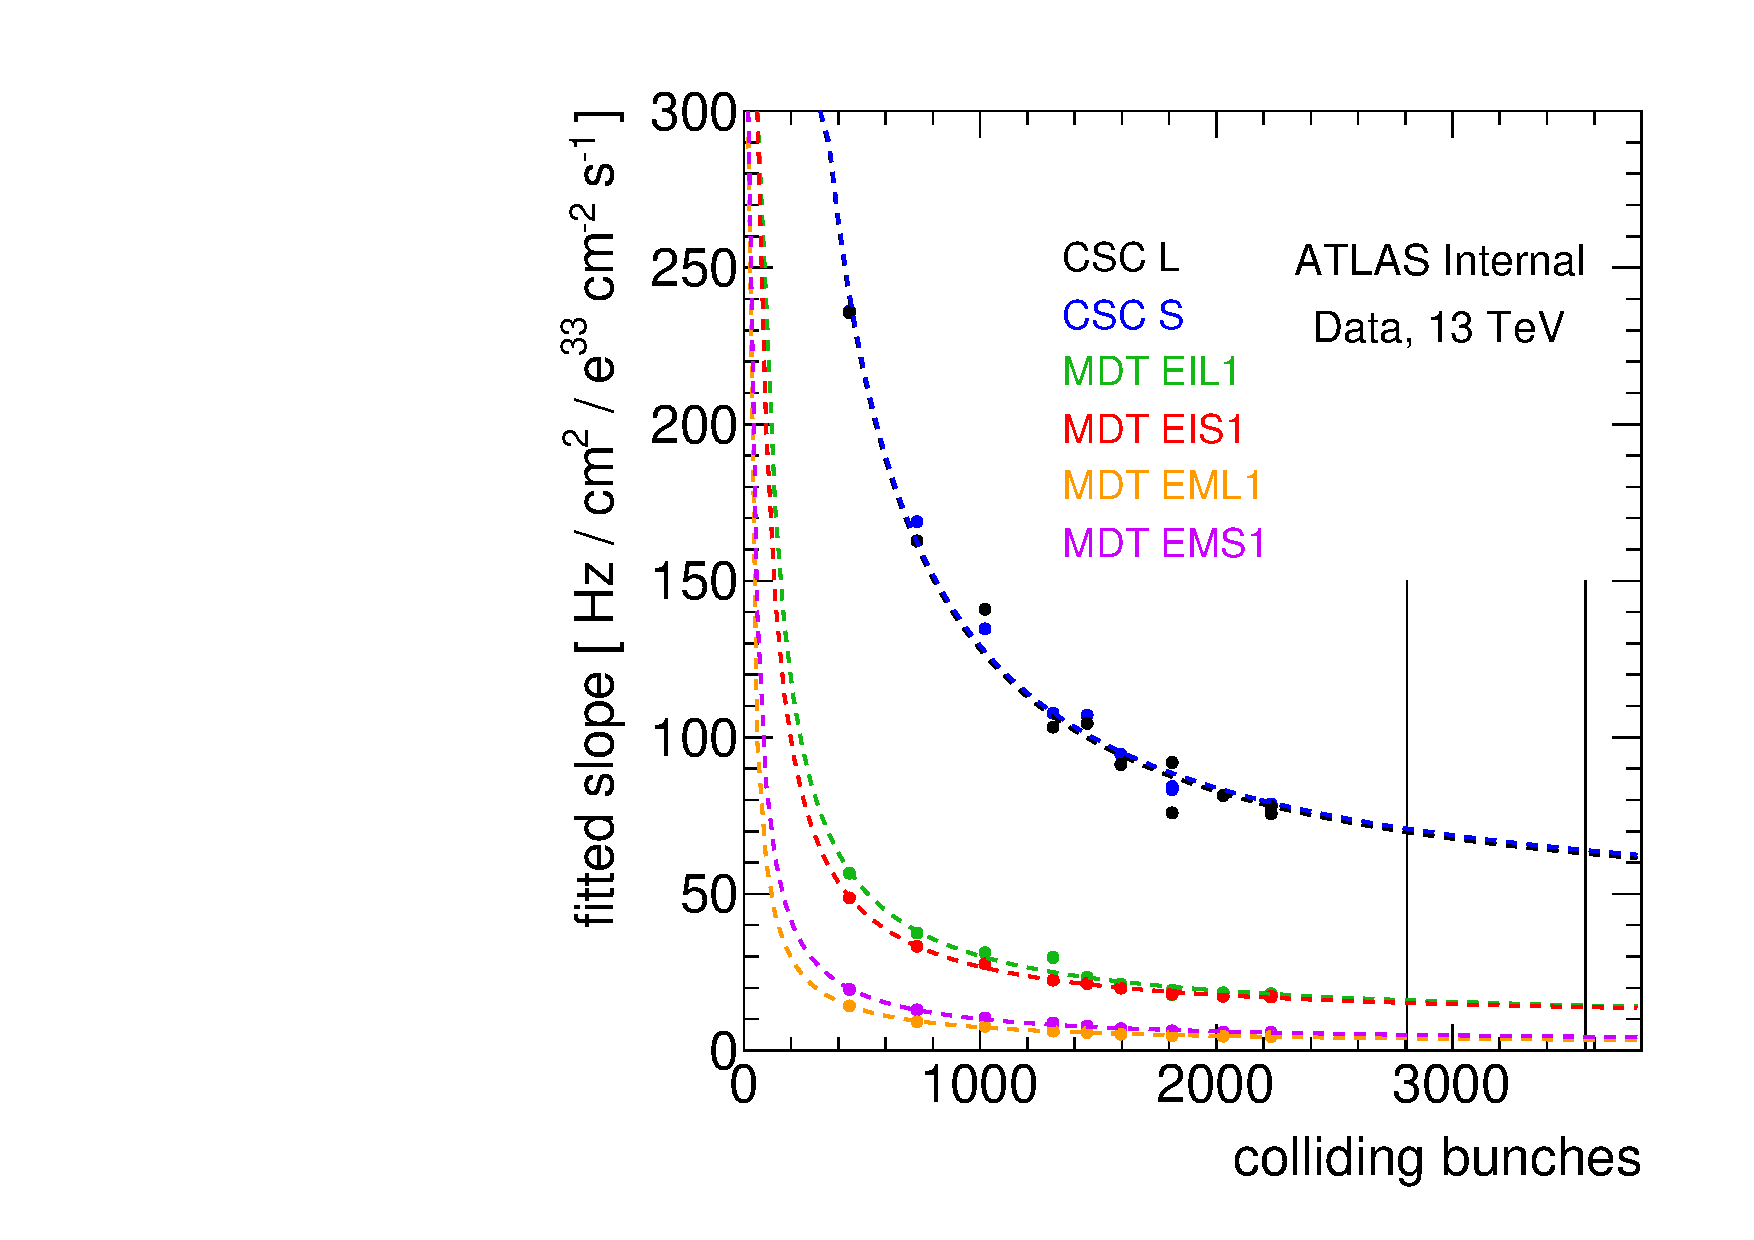
\includegraphics[width=0.45\textwidth]{./figures/slope_vs_bunches_adc_lin.pdf}
    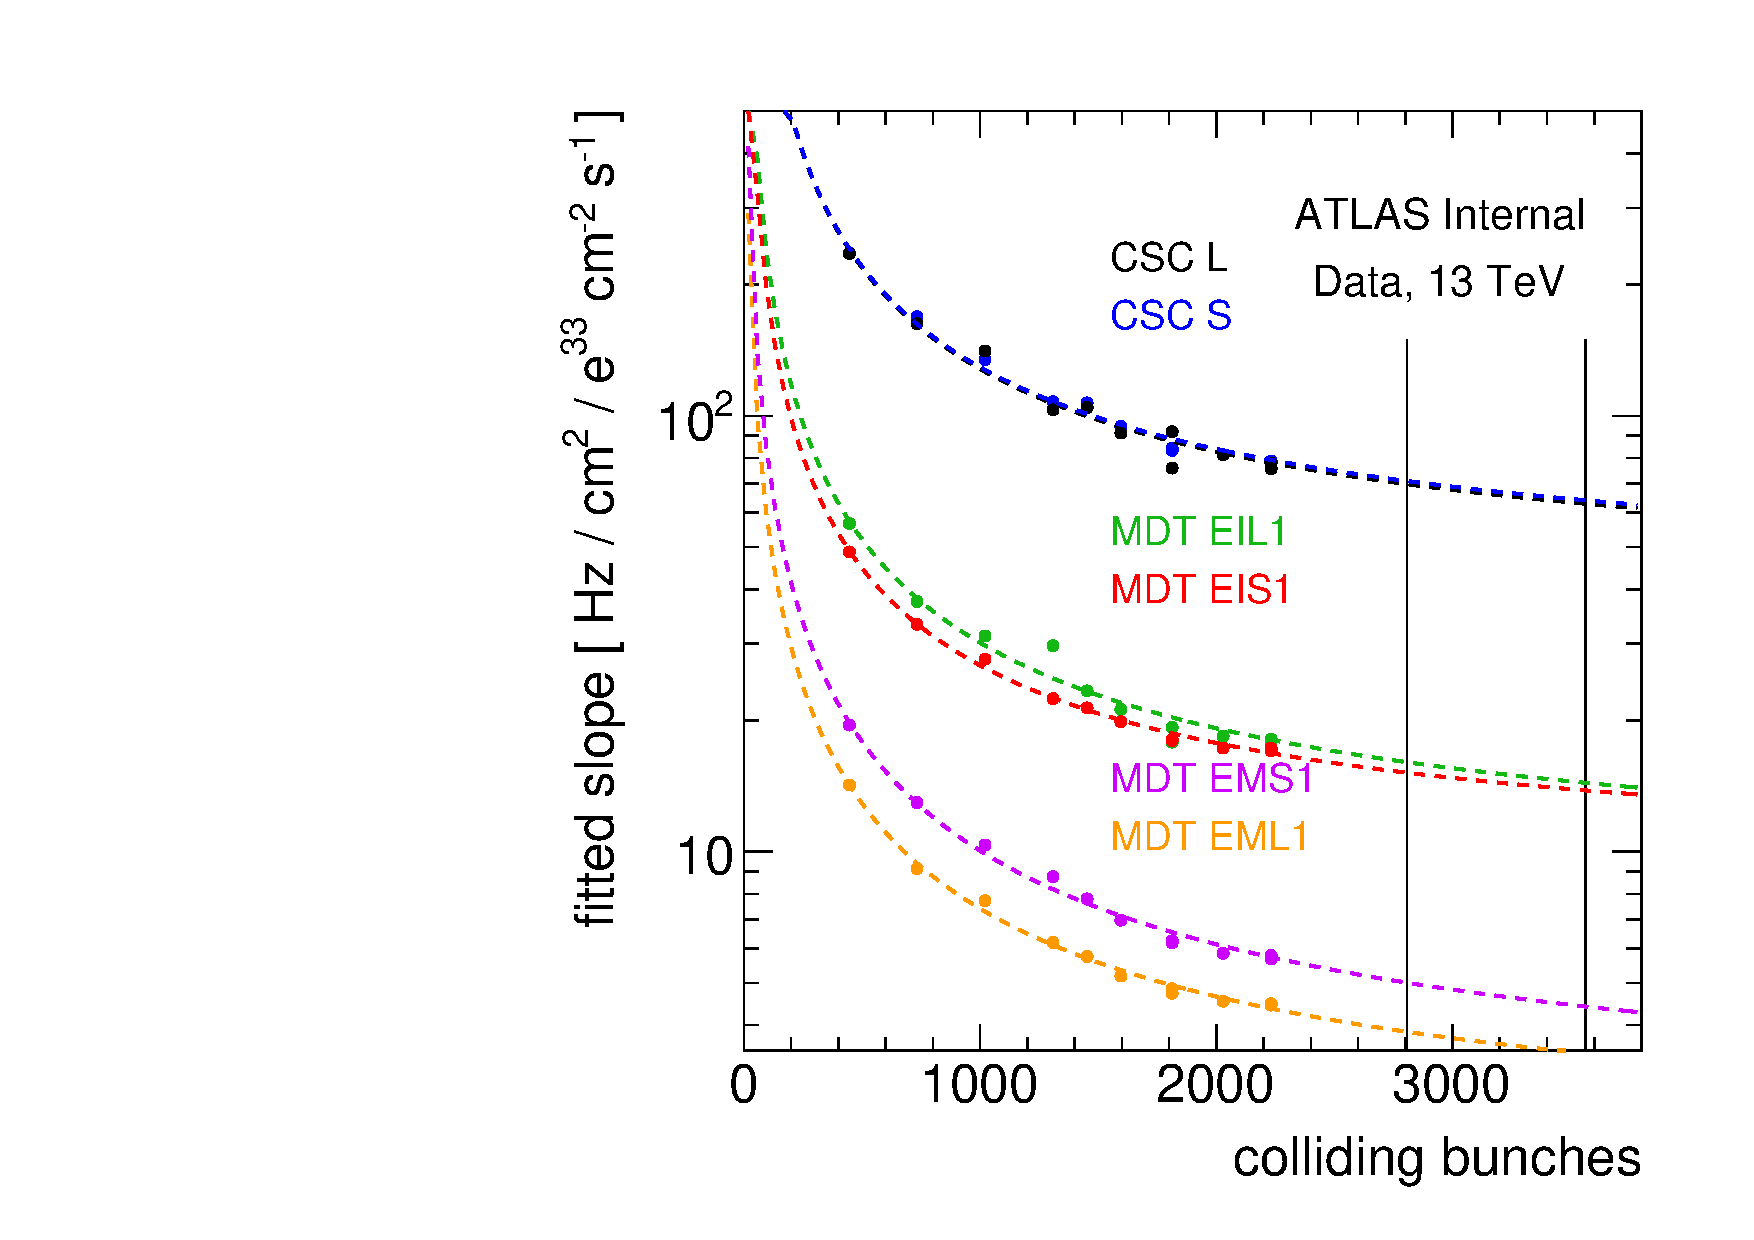
\includegraphics[width=0.45\textwidth]{./figures/slope_vs_bunches_adc_log.pdf}
    \caption{The fitted slope as a function of the number of colliding bunches for various runs in the hottest MDT and CSC chambers, shown with linear (left) and logarithmic (right) scale. The spectra are fitted to $A + B/x$, where $x$ is the number of bunches.}
    \label{fig:extrapolations-slope-vs-bunches-adc}
  \end{center}
\end{figure}

\begin{figure}
  \begin{center}
    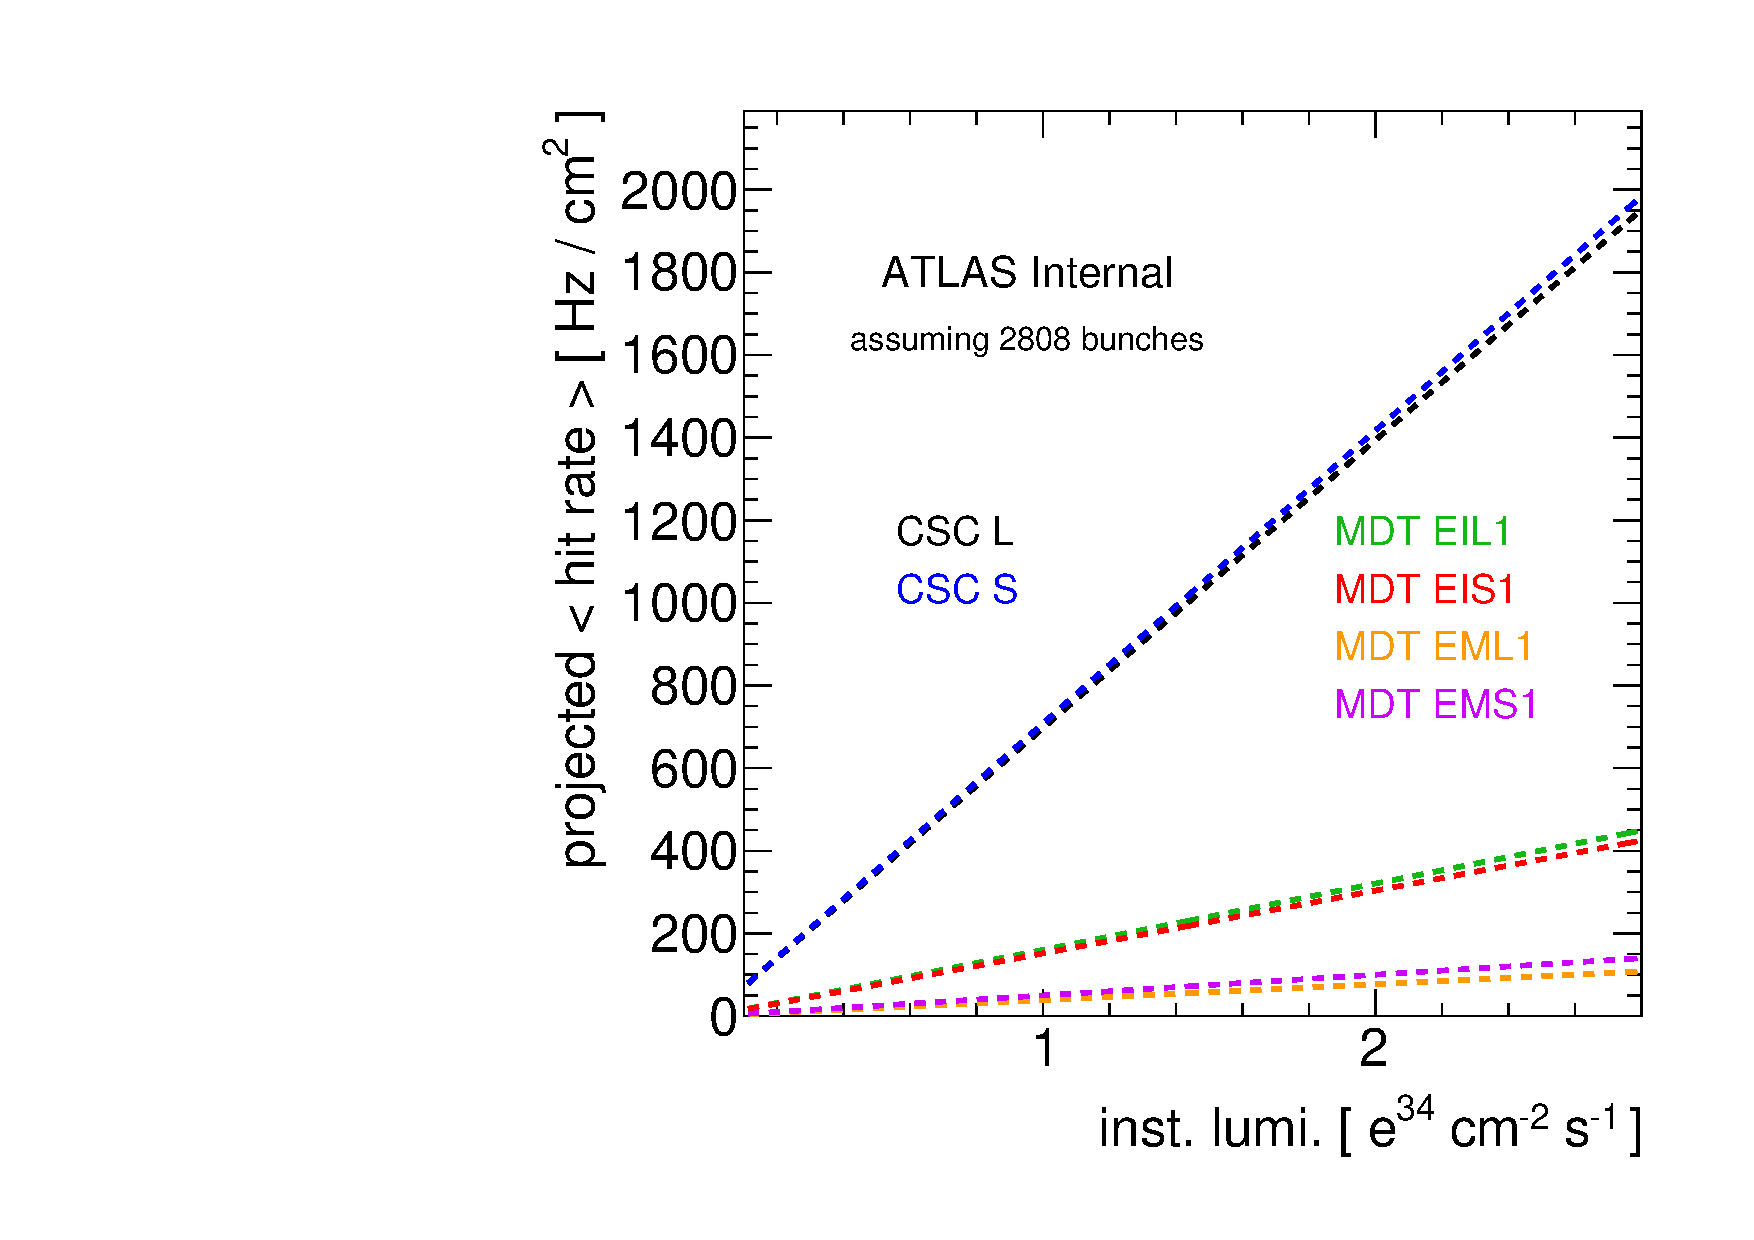
\includegraphics[width=0.45\textwidth]{./figures/extrapolate_vs_lumi_adc_2808.pdf}
    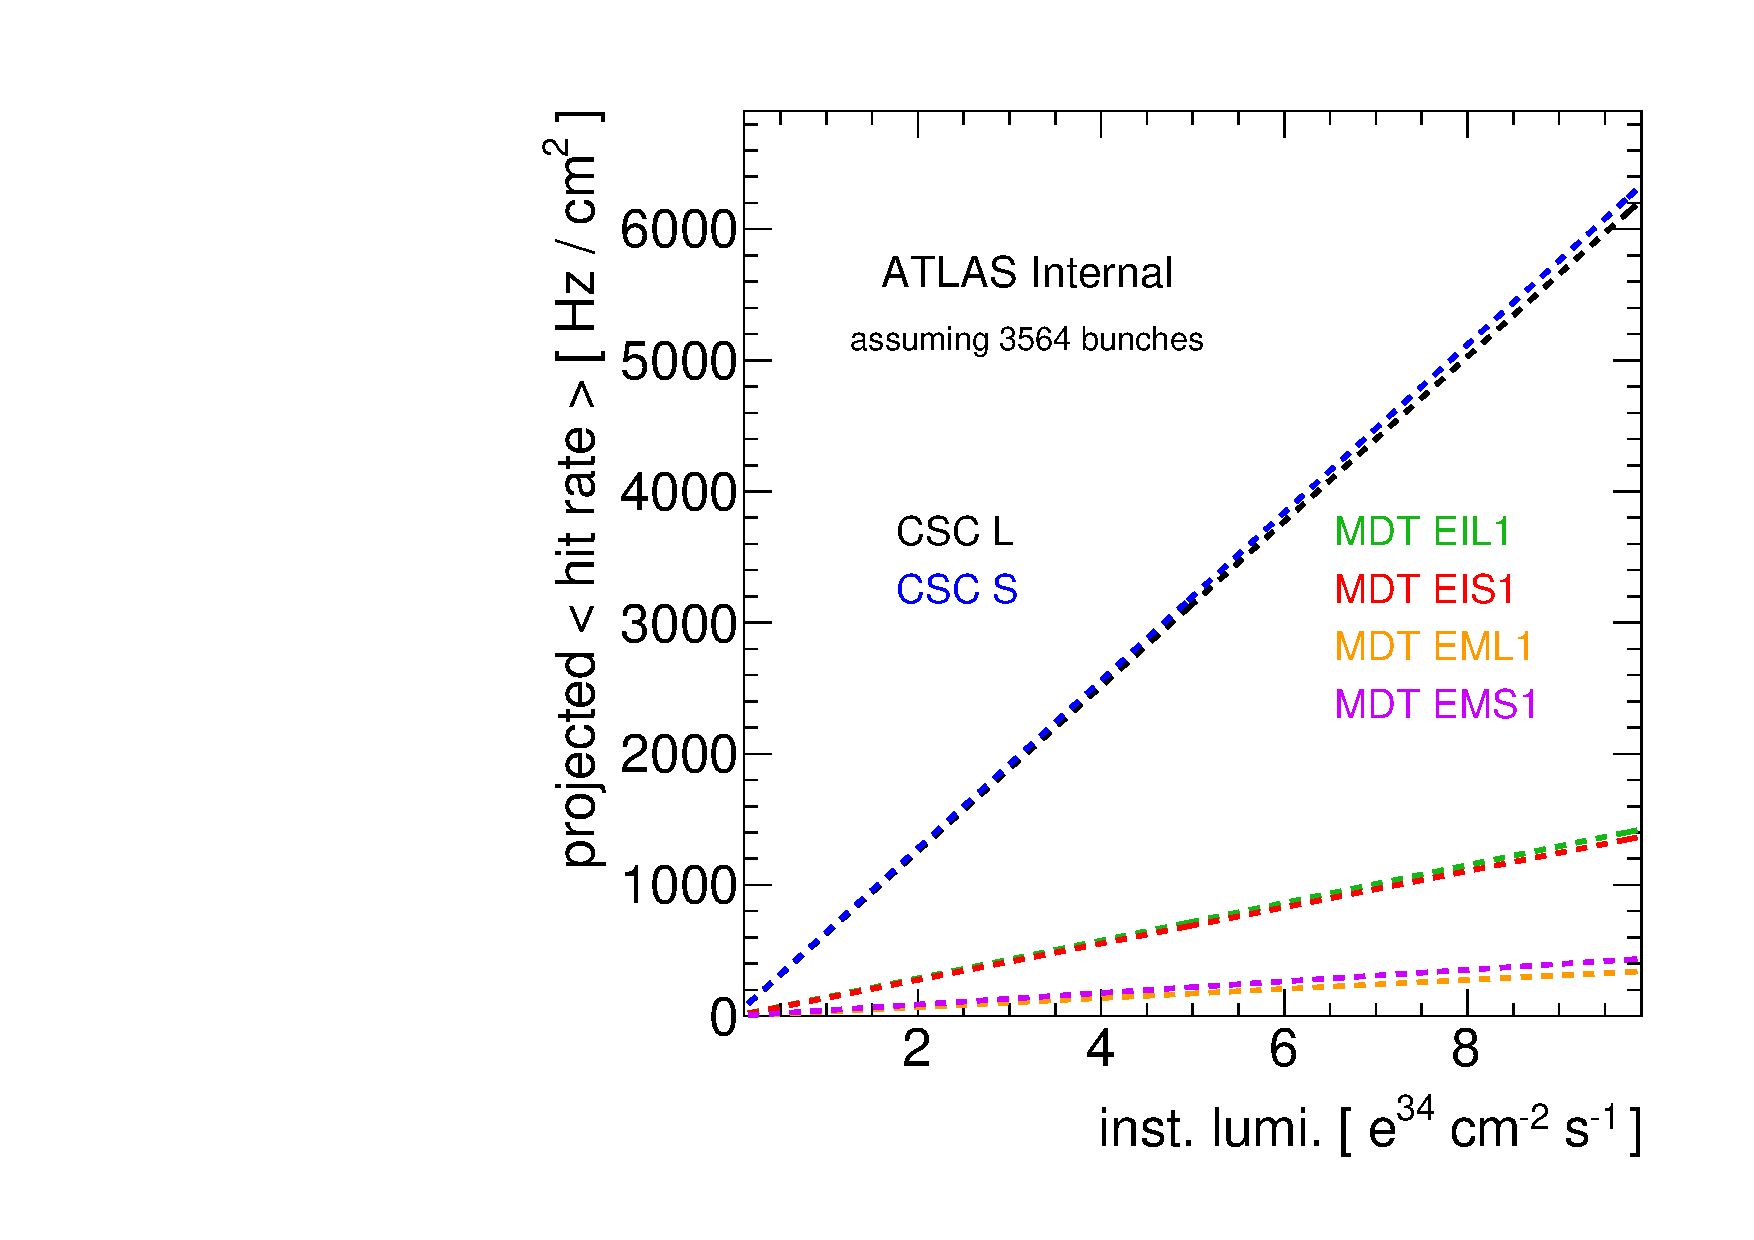
\includegraphics[width=0.45\textwidth]{./figures/extrapolate_vs_lumi_adc_3564.pdf}
    \caption{Projected average hit rates in the MS as a function of instantaneous luminosity, assuming 2808 (left) and 3564 (right) filled bunches in the LHC. The CSC and MDT EI regions are overlaid.}
    \label{fig:extrapolations-hitrates-adc}
  \end{center}
\end{figure}

\begin{table}
  \begin{center}
    \renewcommand{\arraystretch}{1.4}
    \begin{tabular}{c|c|c}
      \multicolumn{1}{c}{} & \multicolumn{2}{c}{\rate} \\
      \hspace{0.6cm}Region\hspace{0.6cm} & \hspace{0.6cm}Run 3\hspace{0.6cm} & HL-LHC   \\
      \hline\hline
      CSC L        & 697.0     & 4399.66 \\
      CSC S        & 708.6     & 4479.66 \\
      \hline
      MDT EIL1     & 160.4     & 1007.13 \\
      MDT EIS1     & 151.8     &  967.57 \\
      \hline
      MDT EML1     &  38.6     &  241.16 \\
      MDT EMS1     &  50.1     &  308.94 \\
    \end{tabular}
    \caption{Projected average hit rates at Run 3 and HL-LHC conditions in the hottest regions of the MS. Run 3 conditions assume $\mathcal{L}=2\times10^{34}$ and 2808 filled bunches in the LHC. HL-LHC conditions assume $\mathcal{L}=7\times10^{34}$ and 3564 filled bunches.}
    \label{tab:extrapolations-hitrates-adc}
  \end{center}
\end{table}

The CSC hit rate in 2015 data-taking closest to the beampipe is 1.94 (2.28) times larger than the average hit rate of the large (small) chambers. This implies the hottest region of the NSW will have a hit rate of between 8535 and 10214 $\text{Hz} / \text{cm}^2$, depending on the number of filled bunches in the LHC, and assuming no changes to the shielding of the MS or the beampipe. The projected hit rates with quality criteria requirements are 10-15\% lower than the inclusive projected hit rates.

